\hspace{1.5cm}The application of machine learning techniques implies a personal and subjective role, namely the selection of the features that can best describe the context of the response variable. The context is not insignificant, it is the most important part of this process. The more valuable the information fed to the algorithm, the more accurate the construction of the model.\\\\
The data used to construct the models in this work was obtained through the site BindingDB.org, which is a database of measured binding affinities of protein considered to be drug-targets (receptors) with small, drug-like molecules (ligands). The database contains experimental information about the binding affinities of 175 inhibitors of the SK4 potassium channel, measured as half-maximal inhibitory concentration ($\text{IC}_{50}$(nM)).\\

\textbullet\hspace{0.1cm} \textbf{$\text{IC}_{50}$}: necessary concentration of the ligand that is necessary to achieve 50\% inhibition of the receptor.\\

The $\text{IC}_{50}$ was in fact the measure that we attempted to model in this work. More precisely, the logarithm of the $\text{IC}_{50}$ (p$\text{IC}_{50}$) was modeled, since we observed that the distribution of the $\text{IC}_{50}$ in our dataset was heavily skewed, which can cause problems when constructing models. Meanwhile, the p$\text{IC}_{50}$ has a much more convenient Gaussian-like distribution, as can be seen in Figure 3.1.\\

\begin{figure}[h]
    \centering
    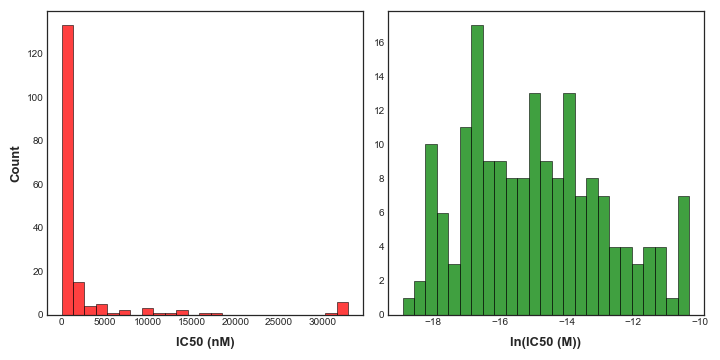
\includegraphics[width=14cm, height=5.7cm]{Images/Results/Feature Analysis/IC50_distributions.png}
    \caption{Histograms of the distributions of the $\text{IC}_{50}$ (left) and its logarithm (right) for the dataset of ligands used in this work.}
\end{figure}

\section{Feature Analysis}
The feature obtaining and management were, as stated, uppermost important parts of this process, as the outcome depends on how  most data is retained whilst being consequent on the significance of each feature. The way to do this guards itself on setting, in some way, how important we want each feature to be, based on the weighing of how relevant it is (positively) to the outcome itself. 

\subsection{Features}
In order to build the models we are interested in, the features extracted beforehand can be divided, broadly speaking, into two groups: features related to the chemical characteristics of the ligands\footnote{These were obtained by the group, the Schrödinger software package was used \cite{maestro}.}, \textbf{chemical features}, and features related to the way in which the bound ligands interact with the receptor protein. These last features can furthermore be divided into \textbf{energetic features} and \textbf{SASA features}.\\

While chemical features were relatively easy to obtain, energetic features such as Van der Waals interactions or hydrogen bonds relating the ligand to the receptor protein, or SASA ($Solvent$-$Accessible$ $Surface$ $Area$) features relating the surface of the receptor accessible to the ligand before and after the linkage, were extracted by the group\footnote{The group used GLIDE software (more information in \cite{glide}).}$^,$\footnote{The group is referred to as in \cite{group}.}. The group performed what is called molecular docking (see Figure 3.2) of the 175 ligands to get the values for these energetic and SASA features. 

\begin{center}
    \begin{figure}[h]
    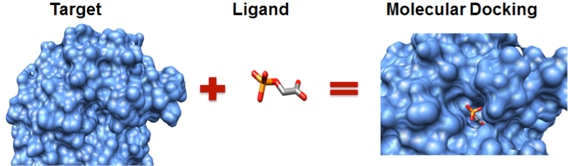
\includegraphics[width=15cm, height=4.5cm]{Images/Results/docking_image.jpg}
    \caption{Schematic illustration of the docking process for a ligand and its target. Image from \cite{docking_figure}.}
    \vspace{-10pt}
    \end{figure}
\end{center}
A total number of 48 descriptor features' data was extracted in the end. More information about some of the most relevant descriptors can be found in the appendix.

\subsection{Feature Conditioning}
Once the selected features' data was collected, PCA was performed on all data to observe how much variance was retained. For this, 17 principal components were obtained; the variance retained can be observed in Figure 3.3.\\\\   

\begin{figure}[h]
    \centering
    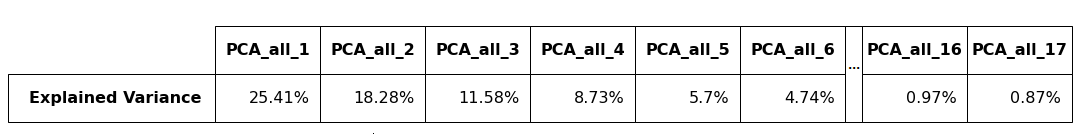
\includegraphics[width=\textwidth]{Images/Results/Feature Analysis/PCA_all variance.png}
    \caption{Observed variance in PCA of all features.}
\end{figure}
In these PCA, it can be assured 95.29\% of all variance was retained, while the first 8 principal components kept 81.6\%. The first 8 principal components were therefore saved, alongside the other 48 features.
As important as it may be holding on to the information on the data, it is also important that irrelevant or repeated data is not given the importance that it does not possess. 
Observing the Pearson correlation among features in Figure 3.4, it can be seen that many of these features are not just almost the same, but can be related to other features in many ways, as some rows (or columns) seem completely identical, and dark quadrants can be spotted in many places, respectively:
\begin{figure}[h]
    \centering
    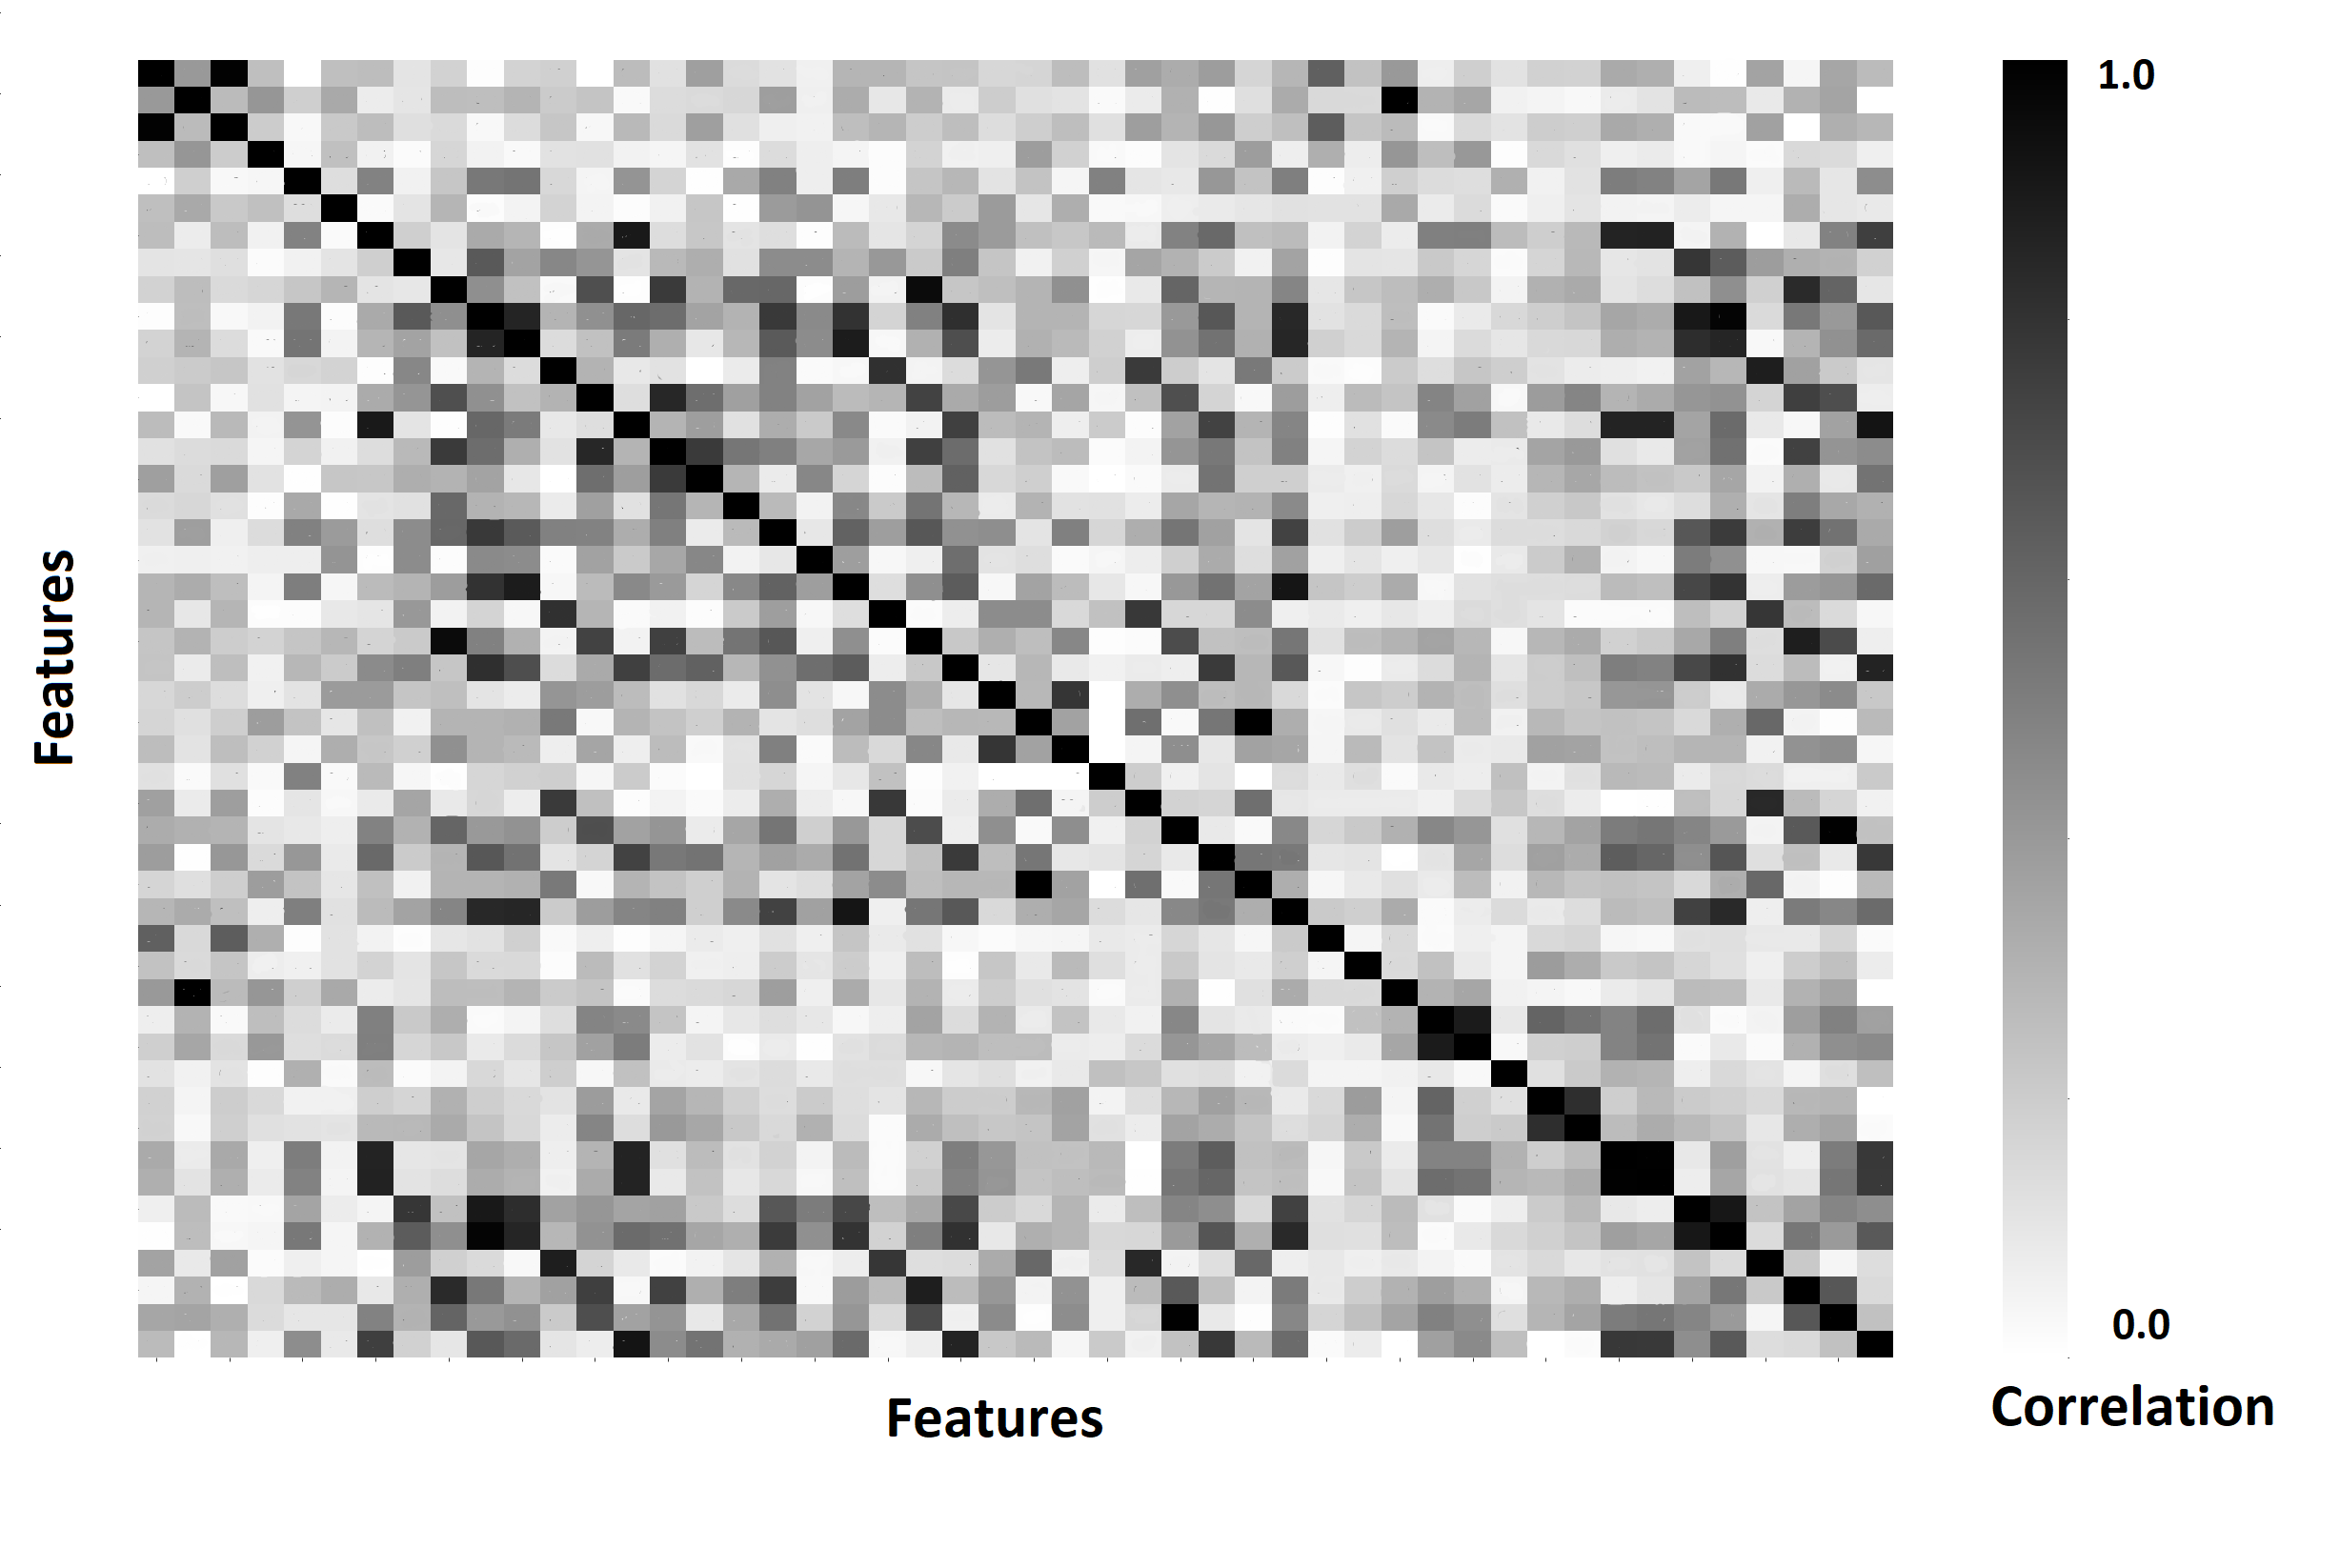
\includegraphics[width=0.6\textwidth]{Images/Results/Feature Analysis/feature correlation.png}
    \caption{Correlation amongst features.}
\end{figure}
\subsection{Feature Clustering}
To identify these correlations better, hierarchical clustering\footnote{It was decided the number of clusters ought to be chosen by a correlation threshold that gave better results, and not beforehand. K-fold clustering was given a try, but no elbow was clear.} was carried on all the features. All the different linkages were examined, as we can see in Table 3.1.
 \begin{table}[h!]
\resizebox{\textwidth}{!}{%
\begin{tabular}{ |p{3.5cm}||p{1.5cm}|p{2.8cm}|p{2.7cm}|p{2.7cm}|p{3.5cm}|  }
 \hline
&Number of\hspace{1cm} clusters &Mean\hspace{1cm} Within-Cluster Correlation&Mean\hspace{1cm} Out-of-Cluster Correlation&Standard\hspace{1cm} Out-of-Cluster Correlation&Number of Unclustered Correlations Above Threshold\\
 \hline
 Ward  linkage   & 13    &0.877856&   0.234071	&0.180442	&5\\
 Single linkage& 9& 0.664165	&0.200436	&0.151496	&0\\
 Complete linkage& 12 & 0.864345	&0.230020	&0.174760&3	\\
 Average linkage& 12 & 0.864345	&0.230020	&0.174760&3	\\
 Centroid linkage& 12  & 0.864345	&0.230020	&0.174760&3	\\
 \hline
\end{tabular}}
\caption{Models and correlations.}
\end{table}





After all the linkage types were explored, one was chosen as well as the appropriate threshold. In Table 3.1, where the obtained feedback for each linkage was obtained, it turns out that single linkage was the worst method (low internal correlation of clusters when creating a single giant cluster). The complete, average and centroid linkage methods obtained the same results, although they arrived at it by different routes. These results seemed slightly better than the Ward linkage, as there were less high correlations outside the cluster, but there was not a huge difference. 
The complete linkage method was chosen, and the dendrogram, as well as the matrix, plotted (Figure 3.5).\\
\begin{figure}[h!]
    \centering
    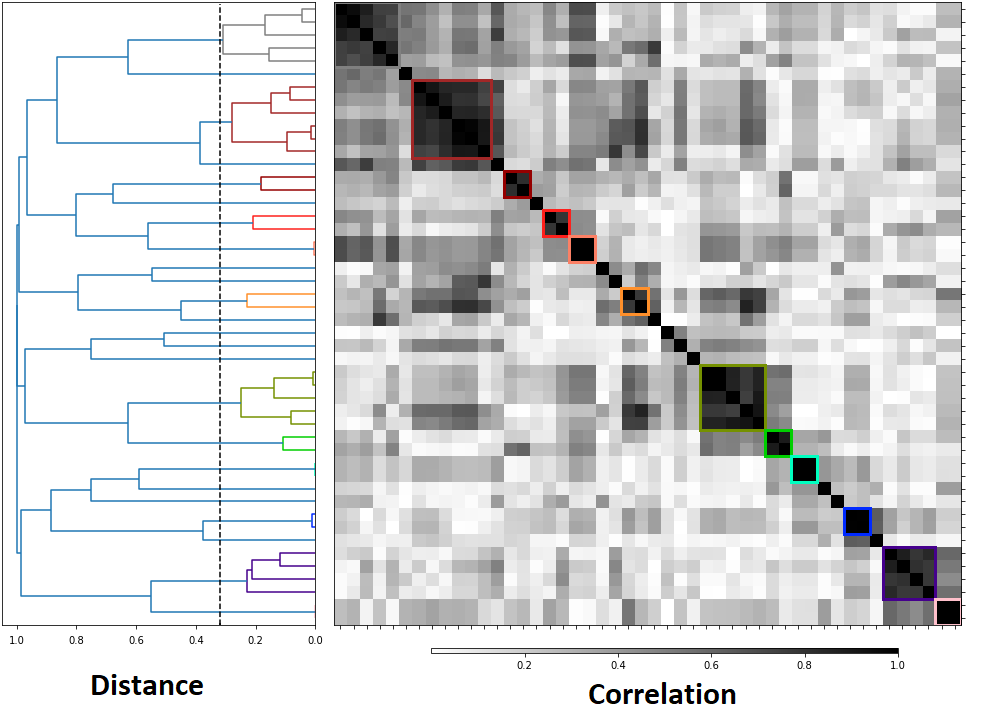
\includegraphics[width=0.8\textwidth]{Images/Results/Feature Analysis/h.complete.png}
    \caption{Complete linkage hierarchical clustering.}
\end{figure}

 Principal component analysis could then be performed on the features of each cluster. The goal was to obtain single features that represent a large percentage of the variance within each cluster. As in Section 3.1.2, the hope was that since a large percentage of the variance was retained, and most of the information of the features within the cluster was represented in these principal components. Clusters with three or more features were taken into account.\\
 \begin{figure}[h!]
    \centering
    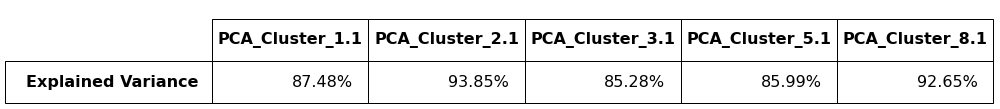
\includegraphics[width=\textwidth]{Images/Results/Feature Analysis/PCA cluster.png}
    \caption{Observed variance in cluster PCA.}
\end{figure} 


 To evaluate the situation with these new features, hierarchical clustering was then performed again. The threshold correlation within clusters was set to 0.68, by having done a grid search around the value, 0.68 was determined to be the most efficient threshold. \\\\
 
\begin{table}[h]
\resizebox{\textwidth}{!}{%
\begin{tabular}{ |p{3.5cm}||p{1.5cm}|p{2.8cm}|p{2.7cm}|p{2.7cm}|p{3.5cm}|  }
 \hline
&Number of\hspace{1cm} clusters &Mean\hspace{1cm} Within-Cluster Correlation&Mean\hspace{1cm} Out-of-Cluster Correlation&Standard\hspace{1cm} Out-of-Cluster Correlation&Number of Unclustered Correlations Above Threshold\\
 \hline
 Ward  linkage   & 13    &0.894085	&  0.228546		&0.187591		&8\\
 Single linkage& 6& 0.578955		&0.174990		&0.138137		&0\\
 Complete linkage& 12 & 0.884122		&0.226165		&0.184679	&8	\\
 Average linkage& 11 & 0.853568	&0.217090		&0.173517	&2	\\
 Centroid linkage& 11  & 0.853568	&0.217090		&0.173517	&2	\\
 \hline
\end{tabular}}
\caption{Models and correlations.}
\end{table}


This is the same as before, but this time the result was the same using the average and centroid linkage methods, and in both cases the number of points with high correlation was minimal as they form larger clusters. This time the centroid linkage method was chosen. The cluster matrix is shown in Figure 3.7. \\

\begin{figure}[h!]
    \centering
    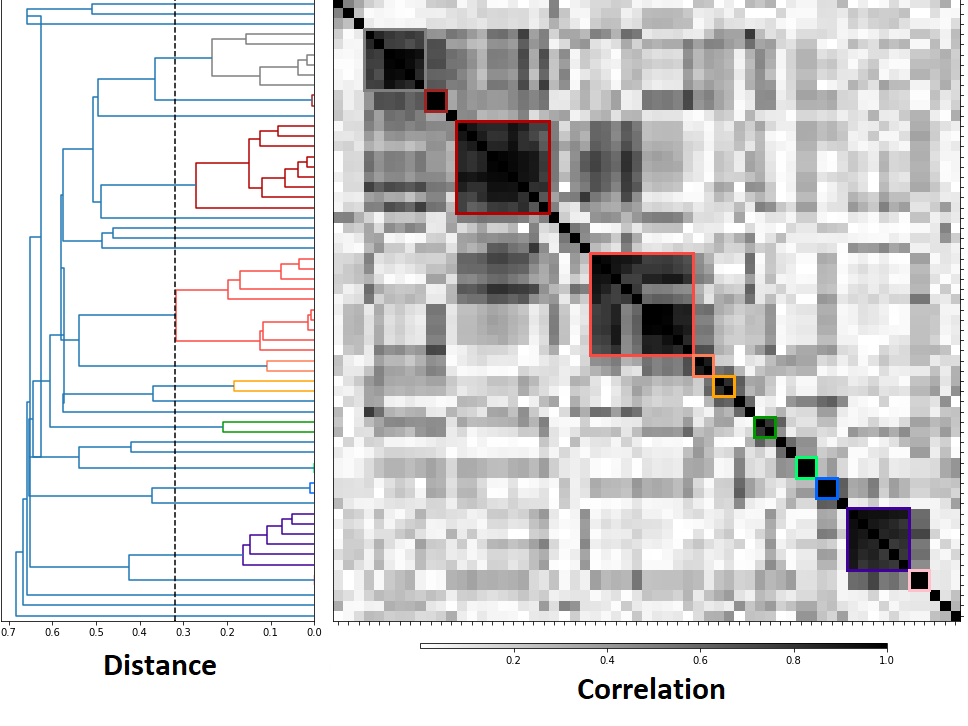
\includegraphics[width=0.8\textwidth]{Images/Results/Feature Analysis/centroid.png}
    \caption{Centroid linkage hierarchical clustering.}
\end{figure}




\subsection{Feature Selection}
These were too many features and a significant correlation could be found among them, so there was need to cut some off because they were only going to overestimate those correlated features.\\\\\\\\

\subsubsection{\hspace{8.85cm}F Score based selection}
\begin{wrapfigure}{l}{0.53\textwidth}
\vspace{-60pt}
\begin{center}
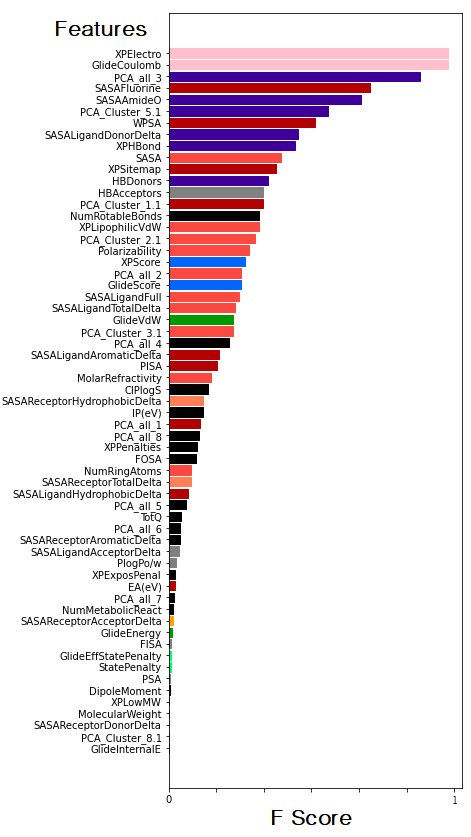
\includegraphics[width=0.50\textwidth]{Images/Results/Feature Analysis/fscore.png}
\caption{\centering Features' F score.}
\vspace{-20pt}
\end{center}
\end{wrapfigure}
For that, the F Scores were calculated for each feature as guides to help choose the best ones from each cluster. In Figure 3.8, the features' F score is observed, where the colour of each bar represents their corresponding cluster.\\

First, one of the of features in each cluster containing only two features was  eliminated. Some features have correlations close to 1, which means they are essentially the same features, so one can just be removed. For pairs of features with lower correlation, the decision was made based on which one has the highest F Score. These scores were calculated over and over again with each removal.
\subsubsection{Cluster correlation based selection}
Second, unnecessary features were eliminated within each cluster. The  correlation matrix of each cluster was plotted, with the goal of keeping as much information within the cluster while removing as many correlations as possible. Decisions were taken based on the F scores as well as the within-cluster correlations.\\

Having removed most of the correlations within the feature set, the correlation matrix (Figure 3.10) was redrawn, and compared to the one with all the features (Figure 3.9).
\begin{figure}[h!]
  \centering
  \begin{minipage}[b]{0.48\textwidth}
    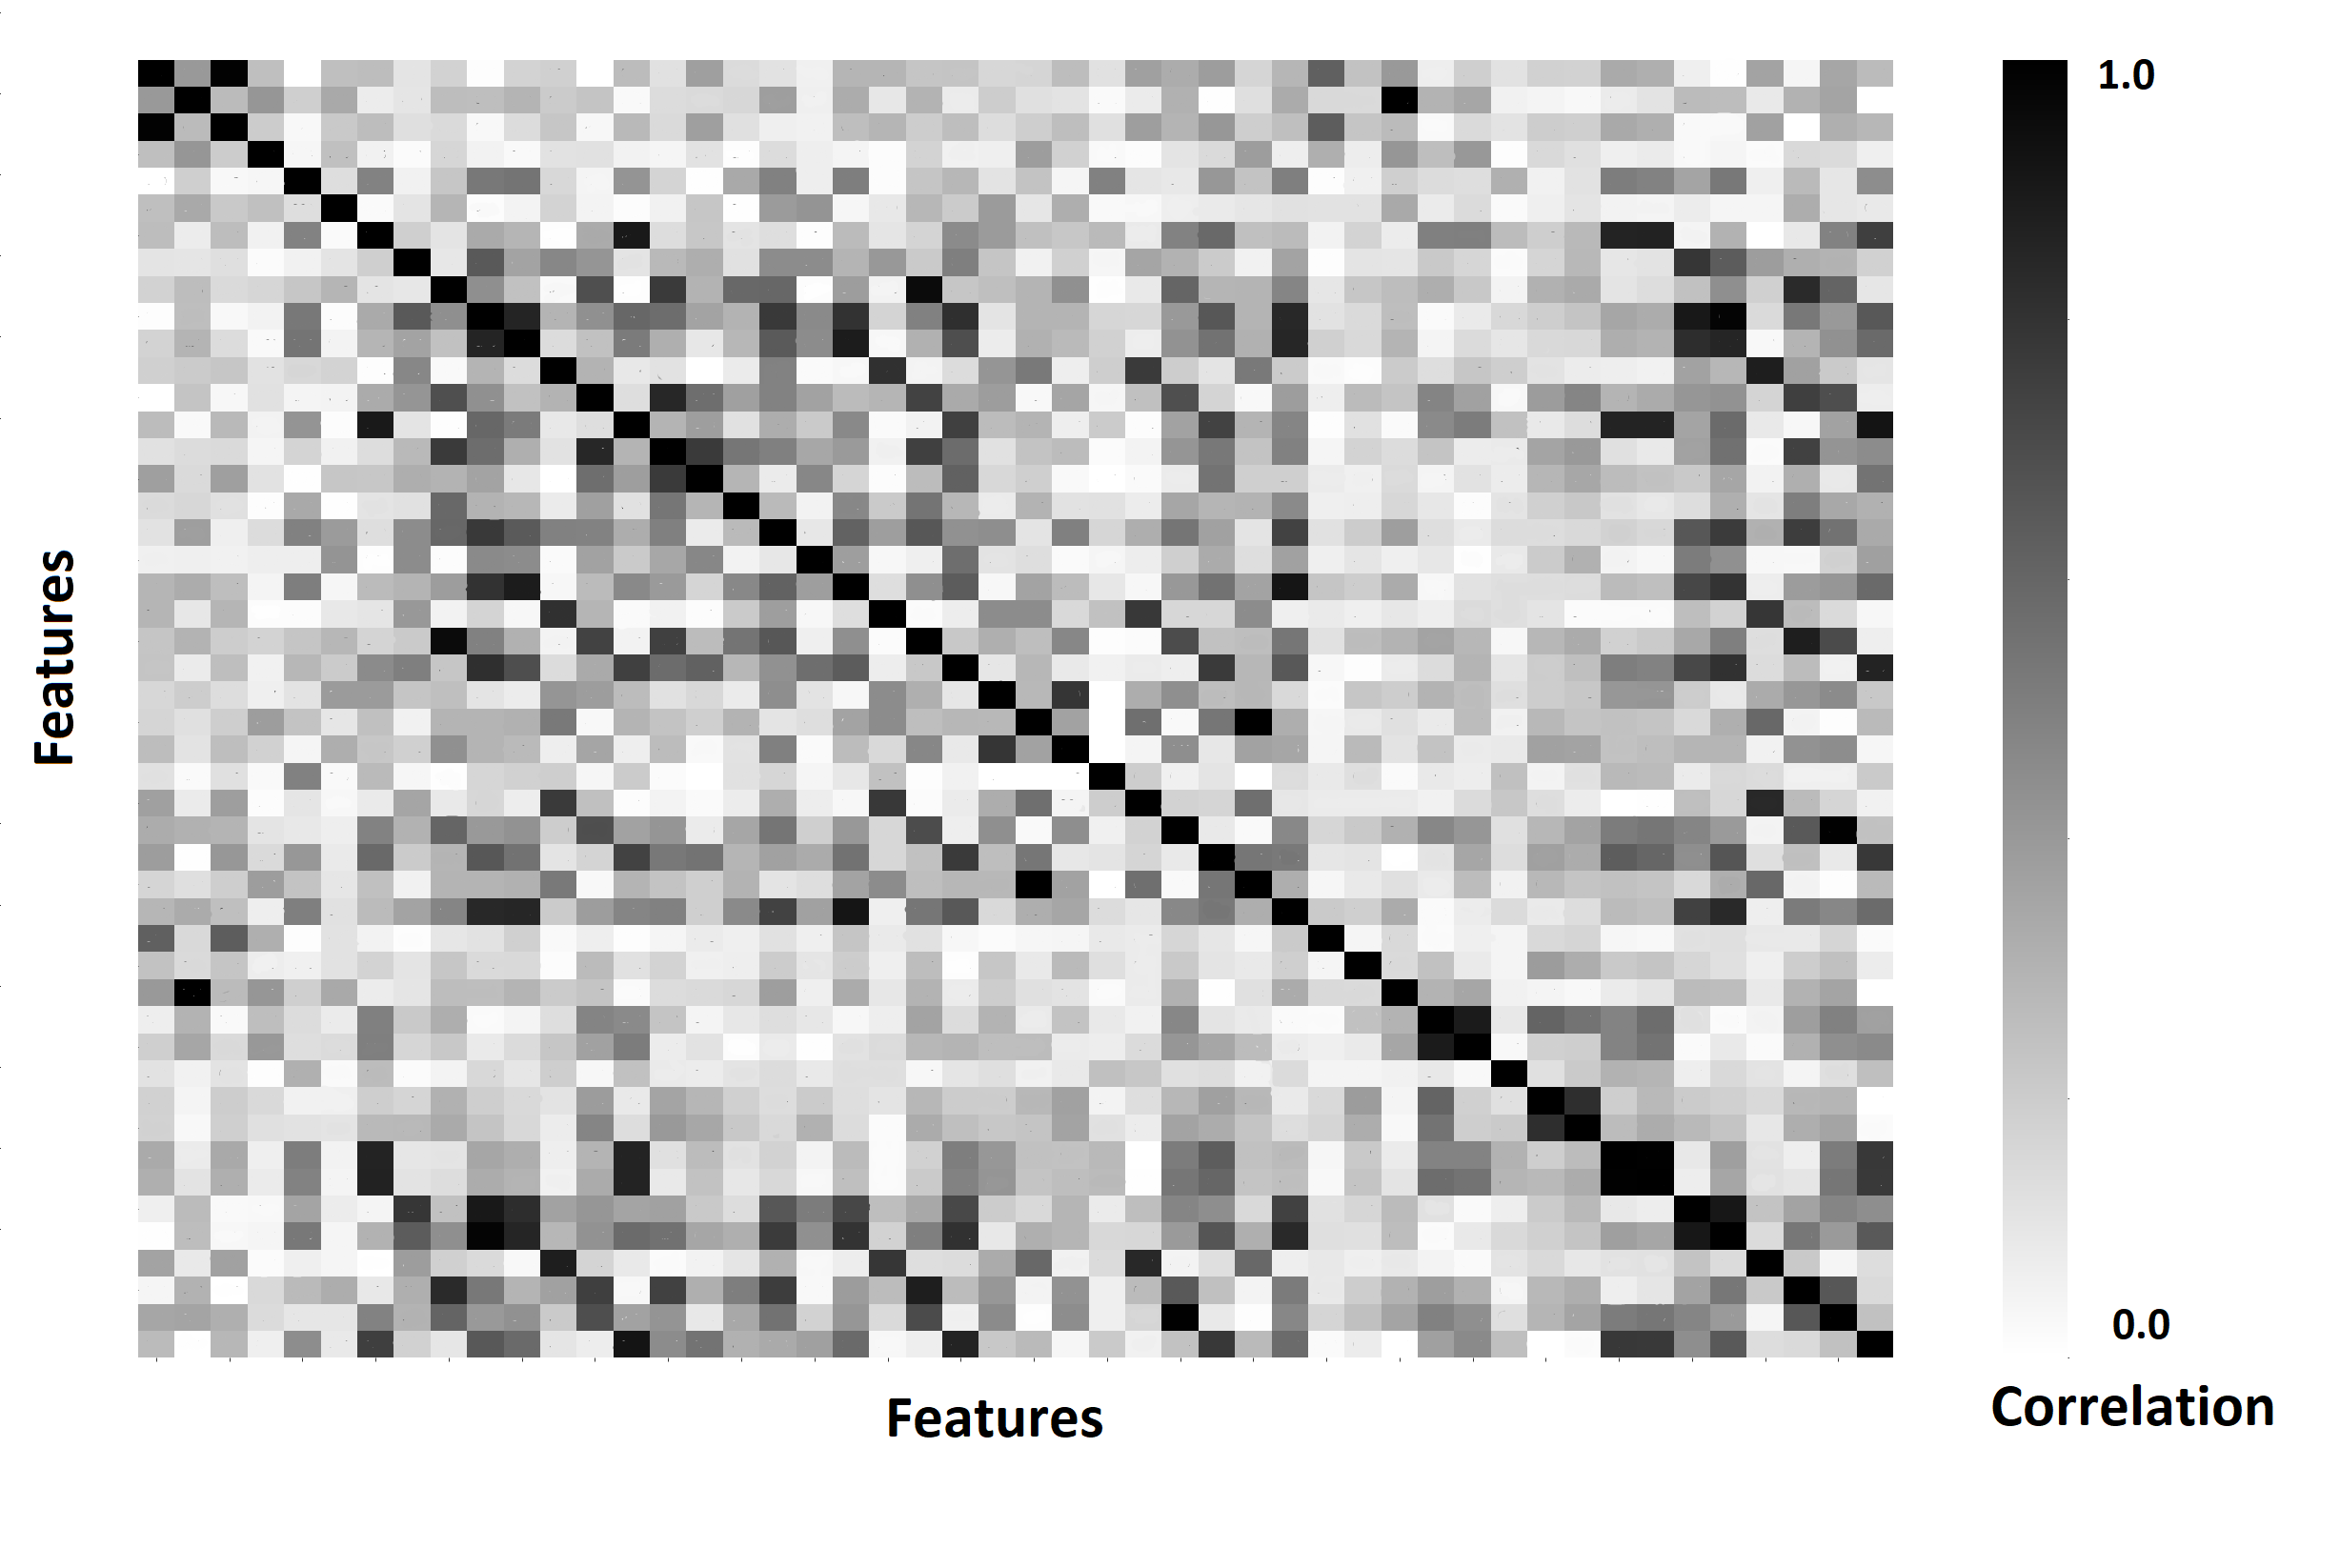
\includegraphics[width=\textwidth, height=5.8cm]{Images/Results/Feature Analysis/feature correlation.png}
    \caption{Correlation before.}
  \end{minipage}
  \hfill
  \begin{minipage}[b]{0.48\textwidth}
    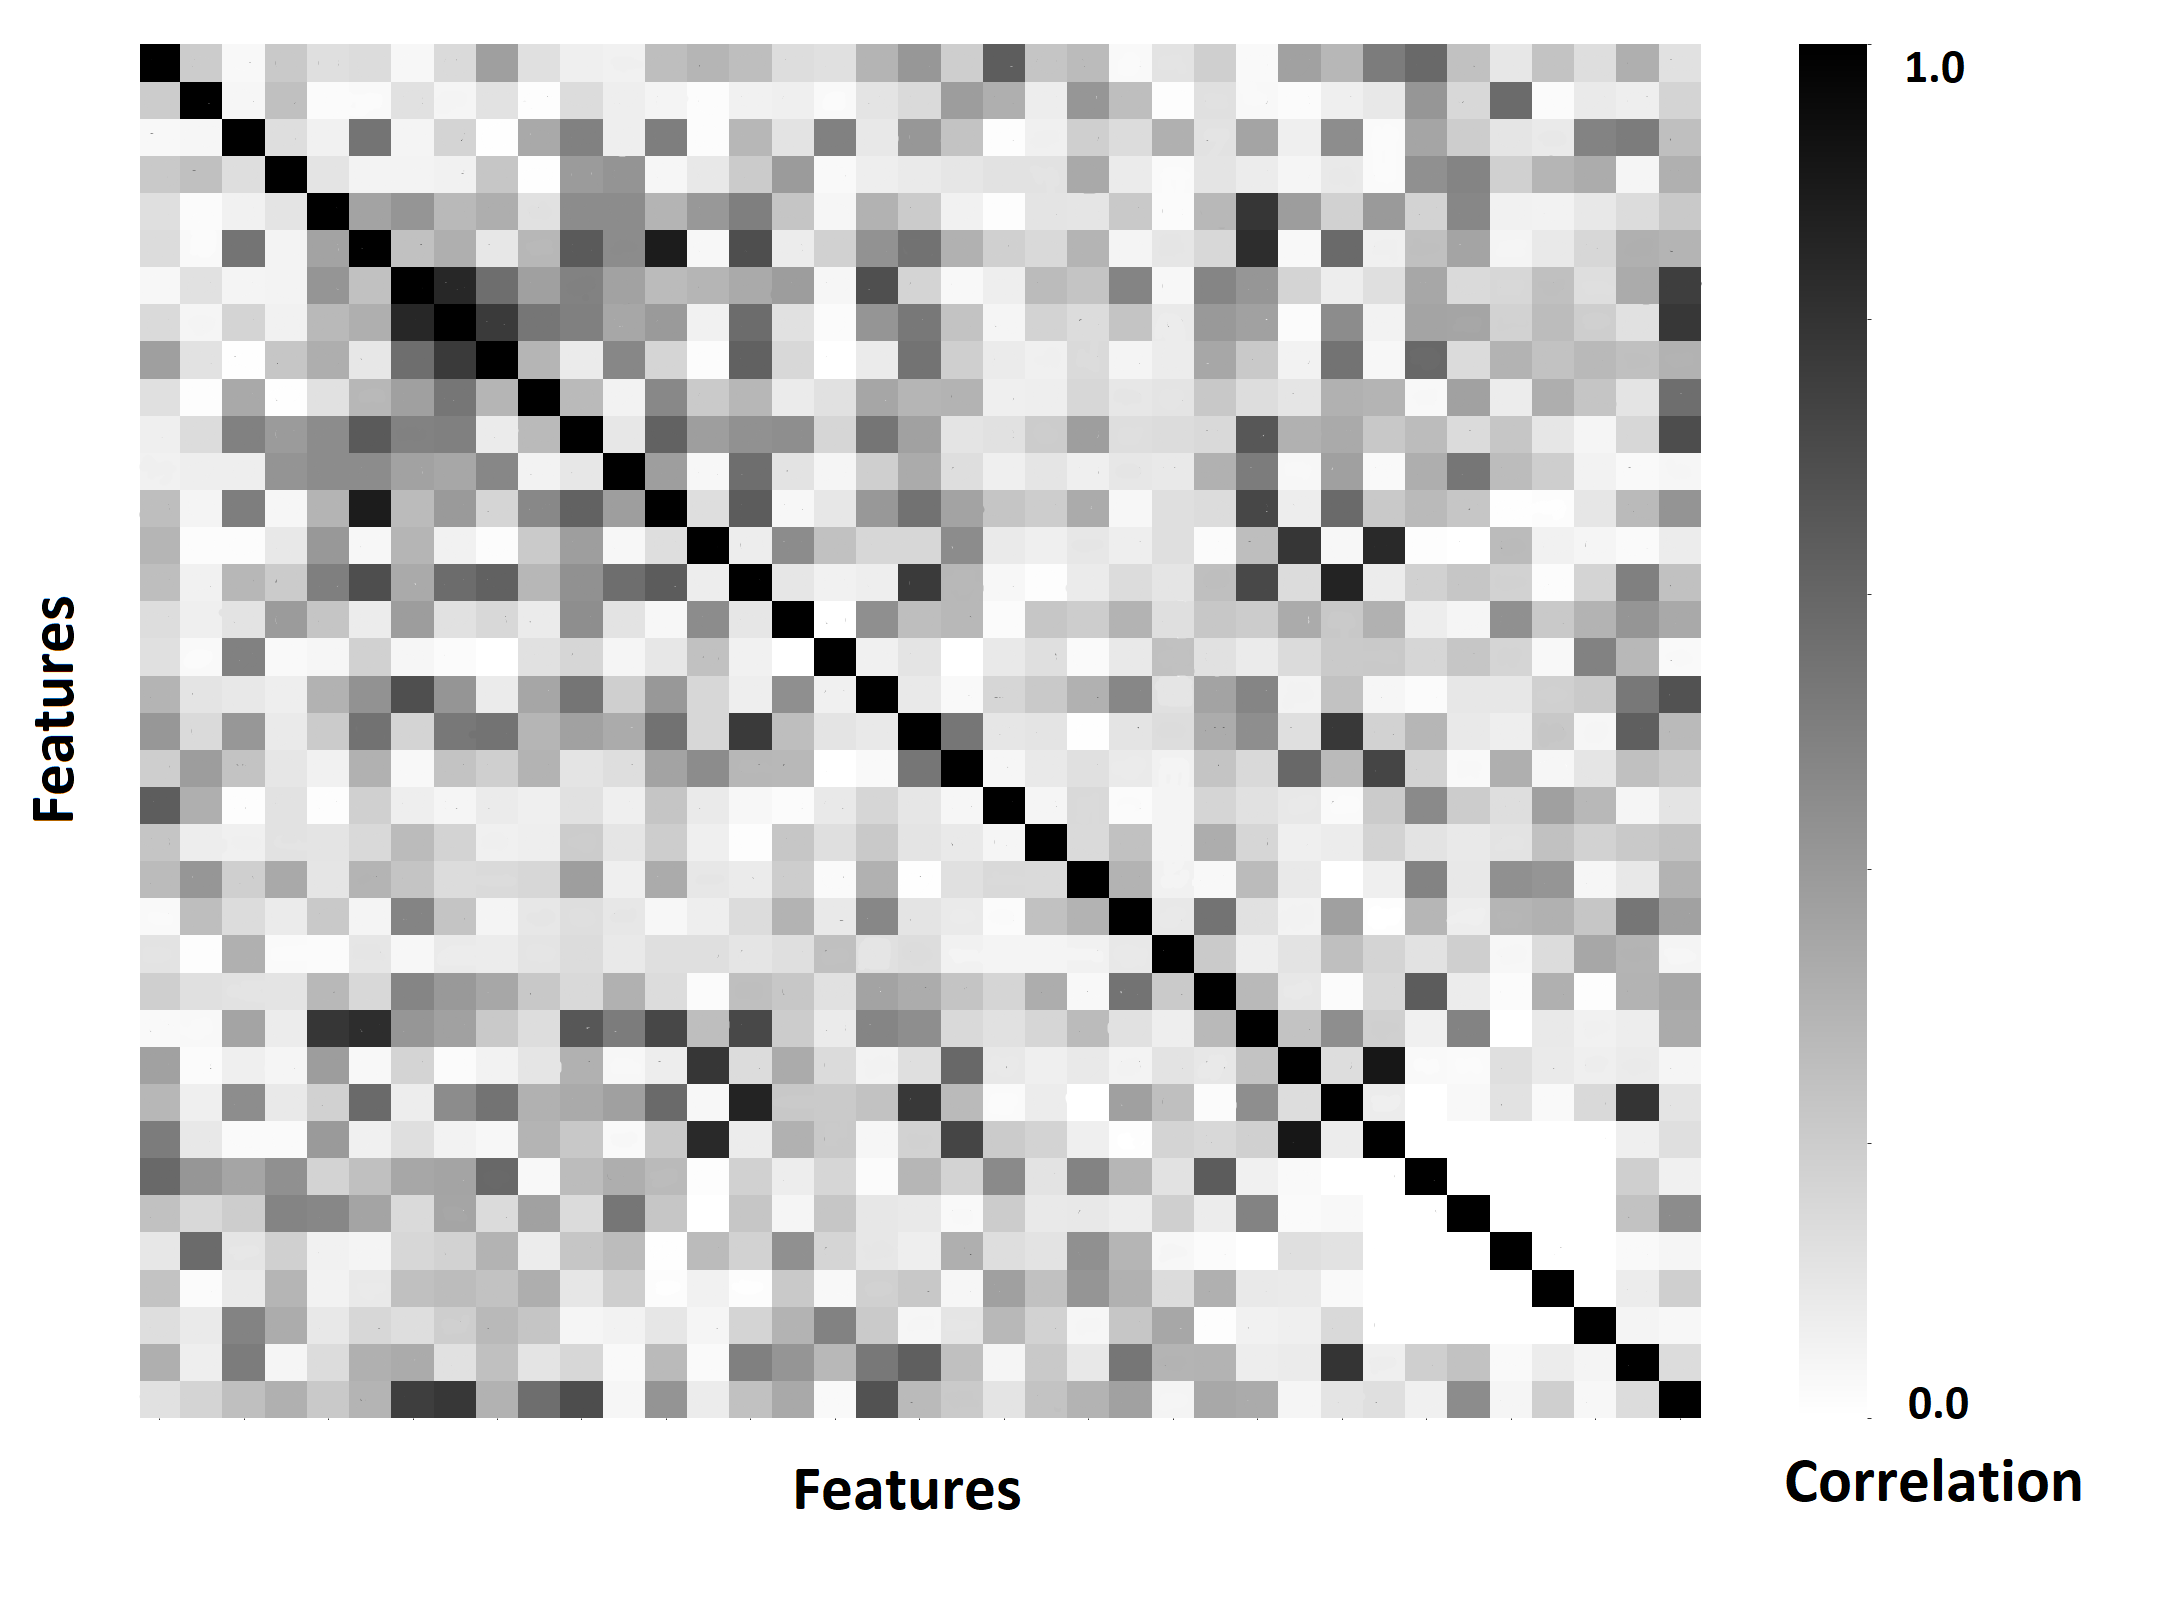
\includegraphics[width=\textwidth]{Images/Results/Feature Analysis/Pearson after.png}
    \caption{Correlation after.}
  \end{minipage}
\end{figure}


\subsubsection{Regressor performance as function of feature number}
Despite the substantial feature reduction, the feature selection algorithm could be used to determine that overfitting was still a problem. Figure 3.11 and Figure 3.12 show the average RMSE for backward feature selection in ridge and Random Forest, respectively.
In these figures, the error drops significantly when most of the relevant features are removed. This is simply due to overfitting, as there are too many features and the observations are not relatively numerous; this does not mean that the features were throwing off the estimation.
\begin{figure}[h!]
    \centering
    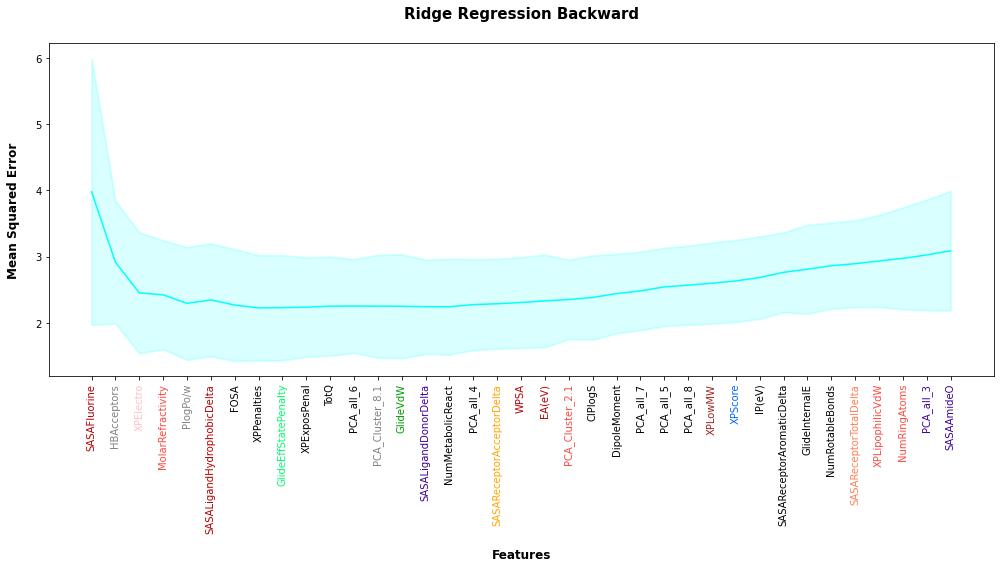
\includegraphics[width=0.8\textwidth]{Images/Results/Ridge Backward.png}
    \caption{Backward feature selection in the ridge regressor.}
\end{figure}
\begin{figure}[h!]
    \centering
    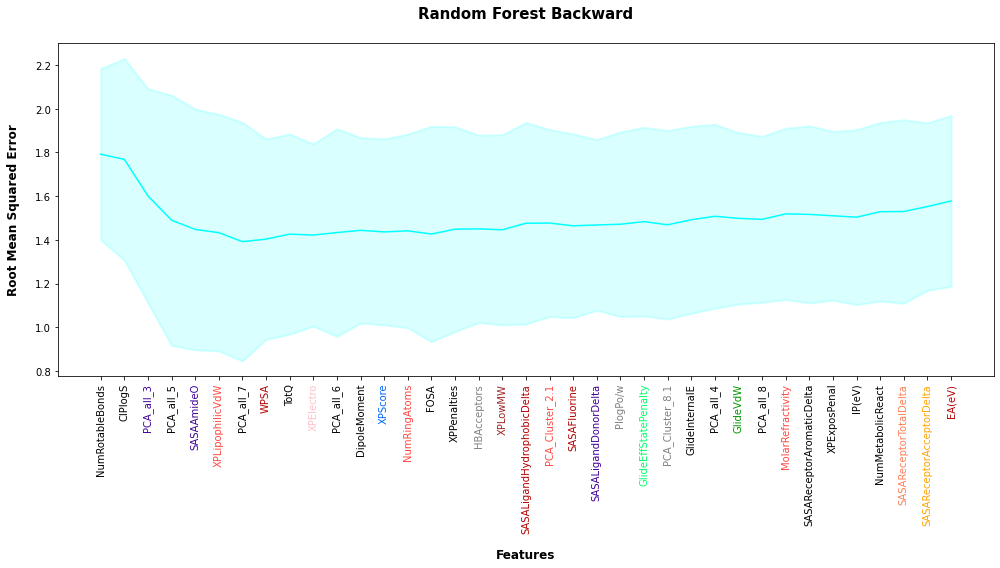
\includegraphics[width=0.8\textwidth]{Images/Results/RF Backward.png}
    \caption{Backward feature selection in the Random Forest regressor.}
\end{figure}

\section{Hyperparameter Optimization}
Once with the feature selection completed, the optimization of hyperparameters of the algorithms to apply (Random Forest and ridge regression) is a very important part. As explained in nested cross-validation, in cases where it wasn't clear which value was the optimal one, a grid search was performed.\\

In the case of \textbf{ridge regression}, the only parameter to optimise was $\alpha$, the regularisation parameter. The learning curve for different values of the regularisation parameter  was plotted (Figure 3.13).

\begin{figure}[h!]
    \centering
    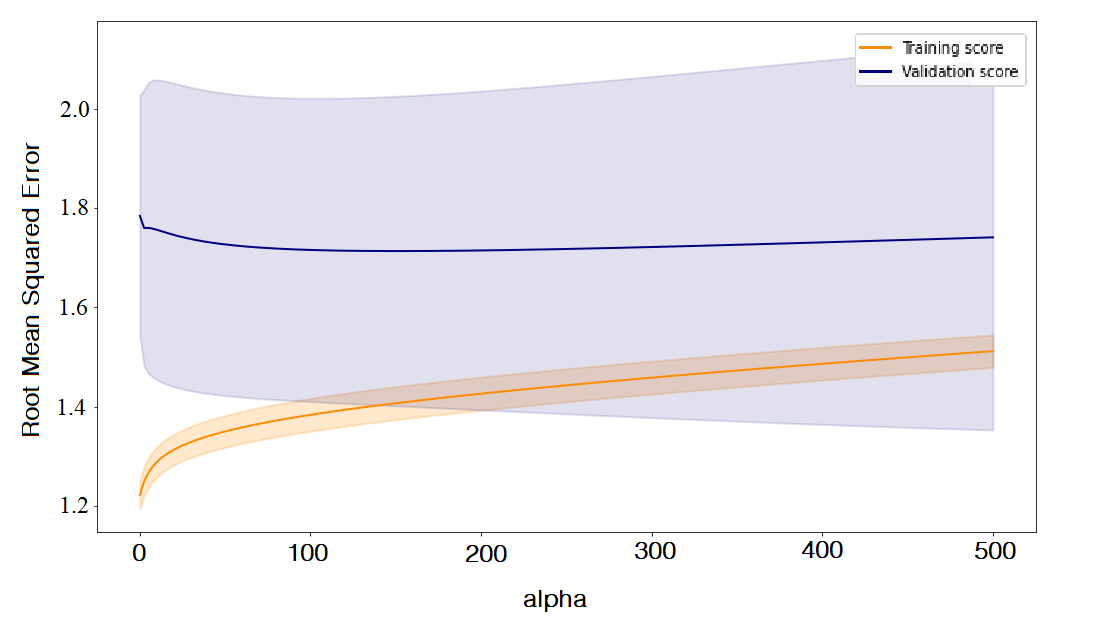
\includegraphics[width=0.8\textwidth]{Images/Results/Hyperparameter/alphalc.png}
    \caption{Learning curves for alpha in ridge regression.}
\end{figure}
It can be seen that the regularization parameter doesn't have a huge impact on the performance of the algorithm, but we can see the a value around 100 might be optimal, which suggests the model is higher variance than it might have seemed.\\

It was decided to do a 250 section grid search from 0 to 125. In the end, the grid search showed inclination towards an unexpectedly small optimal value of $\alpha$ (more in grid search eligibility counts, in the appendix).\\\\

In the case of \textbf{Random Forest}, the hyperparameters which gave out interesting learning curves were firstly, the maximum depth of the decision trees (Figure 3.14); the number of estimators or trees used in the Random Forest; and the maximum number of features taken into account in each tree. This last one was not as important in the end as the distribution was quite homogeneous (more in grid search eligibility counts, in the appendix).\\\\
\begin{figure}
    \centering
    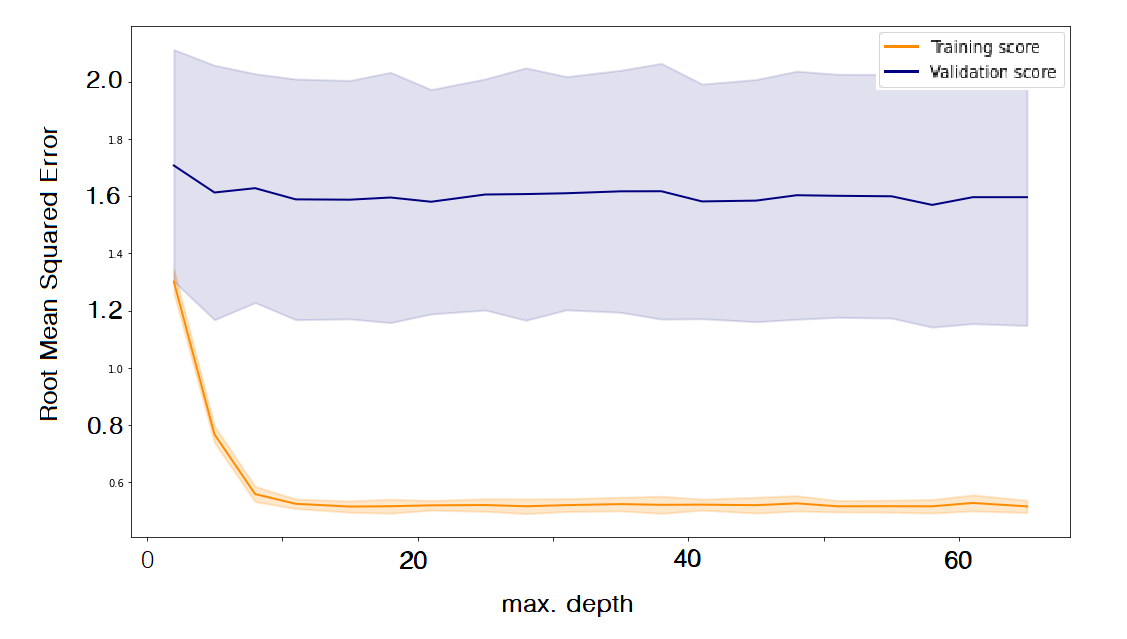
\includegraphics[width=0.8\textwidth]{Images/Results/Hyperparameter/maxdepth.png}
    \caption{Learning curves for maximum depth in Random Forest.}
\end{figure}
Anyhow, a grid search was performed from 1 to 30 in the case of maximum depth; from 25 to 125 with $n$=25 in the number of estimators; and from 0.1 to 1 with $n$=20 in the ratio of maximum features with respect to the total number of features. 


\section{Results}

\subsection{General Evaluation}
After performing nested cross-validation (see Figure 2.11) for each and every regression and correlation metric explained, the obtained values for ridge and Random Forest regression can be visualised in Tables 3.3 and 3.4, respectively.
\begin{table}[h]
\resizebox{\textwidth}{!}{%
\begin{tabular}{l|cccllll|}
\cline{2-8}
                                                   & \multicolumn{1}{l}{\textbf{MAE}}                         & \multicolumn{1}{l}{\textbf{RMSE}}                        & \multicolumn{1}{l}{\textbf{MAPE}}                        & \multicolumn{1}{l}{\textbf{$\rho_p$}}                   & \multicolumn{1}{l}{\textbf{$R^2$}}                       & \multicolumn{1}{l}{\textbf{$\rho_s$}}                    & \multicolumn{1}{l|}{\textbf{$\tau$}}                     \\ \hline
\multicolumn{1}{|l|}{\textbf{Mean}}                & \cellcolor{\color[HTML]{212121} 1.23}      & \cellcolor{\color[HTML]{212121} 2.39}      & \cellcolor{\color[HTML]{212121} 0.085}     & \cellcolor{\color[HTML]{212121} 0.66}     & \cellcolor{\color[HTML]{212121} 0.36}      & \cellcolor{\color[HTML]{212121} 0.61}      & \cellcolor{\color[HTML]{212121} 0.48}      \\
\multicolumn{1}{|l|}{\textbf{95\% CI Mean}}        & \cellcolor{\color[HTML]{212121} 1.18-1.28} & \cellcolor{\color[HTML]{212121} 2.19-2.64} & \cellcolor{\color[HTML]{212121} 0.08-0.09} & \cellcolor{\color[HTML]{212121} 0.61-0.7} & \cellcolor{\color[HTML]{212121} 0.26-0.43} & \cellcolor{\color[HTML]{212121} 0.56-0.66} & \cellcolor{\color[HTML]{212121} 0.43-0.52} \\
\multicolumn{1}{|l|}{\textbf{Standard Error Mean}} & \cellcolor{\color[HTML]{212121} 0.026}     & \cellcolor{\color[HTML]{212121} 0.11}      & \cellcolor{\color[HTML]{212121} 0.0019}    & \cellcolor{\color[HTML]{212121} 0.023}    & \cellcolor{\color[HTML]{212121} 0.044}     & \cellcolor{\color[HTML]{212121} 0.024}     & \cellcolor{\color[HTML]{212121} 0.022}     \\
\multicolumn{1}{|l|}{\textbf{Median}}              & \cellcolor{\color[HTML]{212121} 1.22}      & \cellcolor{\color[HTML]{212121} 2.33}      & \cellcolor{\color[HTML]{212121} 0.086}     & \cellcolor{\color[HTML]{212121} 0.69}     & \cellcolor{\color[HTML]{212121} 0.38}      & \cellcolor{\color[HTML]{212121} 0.64}      & \cellcolor{\color[HTML]{212121} 0.50}      \\
\multicolumn{1}{|l|}{\textbf{Minimum}}             & \cellcolor{\color[HTML]{212121} 0.71}      & \cellcolor{\color[HTML]{212121} 0.81}      & \cellcolor{\color[HTML]{212121} 0.051}     & \cellcolor{\color[HTML]{212121} 0.12}     & \cellcolor{\color[HTML]{212121} -0.68}     & \cellcolor{\color[HTML]{212121} 0.15}      & \cellcolor{\color[HTML]{212121} 0.089}     \\
\multicolumn{1}{|l|}{\textbf{Maximum}}             & 1.71                                                     & 5.00                                                     & 0.13                                                     & 0.90                                                    & 0.79                                                     & 0.89                                                     & 0.77                                                     \\ \hline
\end{tabular}}
\caption{Metrics obtained in the ridge nested CV.}
\end{table}

\begin{table}[h]
\resizebox{\textwidth}{!}{%
\begin{tabular}{l|ccccccc|}
\cline{2-8}
                                                   & \textbf{MAE} & \textbf{RMSE} & \textbf{MAPE} & $\rho_p$  & $R^2$     & $\rho_s$  & $\tau$    \\ \hline
\multicolumn{1}{|l|}{\textbf{Mean}}                & 1.06         & 1.99          & 0.074         & 0.75      & 0.51      & 0.69      & 0.55      \\
\multicolumn{1}{|l|}{\textbf{95\% CI Mean}}        & 1.01-1.12    & 1.75-2.32     & 0.07-0.08     & 0.71-0.78 & 0.43-0.56 & 0.65-0.73 & 0.51-0.58 \\
\multicolumn{1}{|l|}{\textbf{Standard Error Mean}} & 0.030        & 0.15          & 0.0024        & 0.017     & 0.033     & 0.019     & 0.017     \\
\multicolumn{1}{|l|}{\textbf{Median}}              & 1.07         & 1.72          & 0.071         & 0.78      & 0.56      & 0.70      & 0.55      \\
\multicolumn{1}{|l|}{\textbf{Minimum}}             & 0.74         & 0.93          & 0.048         & 0.42      & -0.44     & 0.37      & 0.26      \\
\multicolumn{1}{|l|}{\textbf{Maximum}}             & 1.68         & 5.25          & 0.13         & 0.96      & 0.85      & 0.97      & 0.88      \\ \hline
\end{tabular}}
\caption{Metrics obtained in the Random Forest nested CV.}
\end{table}
Comparing these two tables filled with results, it can be clearly deduced, mainly from the confidence interval section, the results in Random Forest are not only a lot better when it comes to regression error which is lower, but also the correlation metrics seem to be up by a notch. The mean values are also quite better, and the median, which is a good indicator, shows the clear inclination towards improvement.\\\\
\noindent\fbox{%
    \parbox{\textwidth}{%
        It must be said that this enhancement from a simple linear model to a complex non-linear ensemble model such as Random Forest comes at cost in every situation possible, it can be considered universal because of all the distinct metrics used and, therefore, all the scenarios explored. These metrics account for all possible situations, either where there can be outliers in the data or where the data is very trustworthy.
    }%
}
\subsection{Null Hypothesis}
Even after having compared with a ridge regression, the null hypothesis has to be discarded. For this, a so called dummy regressor which estimates the mean of all features' observations and its corresponding RMSE was compared to the actual model and its RMSE. A t-test was performed to check that the obtained performance was statistically significantly different compared to this dummy regressor that always predicts the mean. The null hypothesis is that both models have the same performance (mean RMSE is equal).\\

The t statistic was computed and the p-value was then obtained. This was then compared to the significance $\alpha$, which was chosen to be 0.05. The results obtained were the following:\\
\textbullet\hspace{0.5cm} t statistic: 7.486.\\
\textbullet\hspace{0.5cm} p value: 6.721e-04.\\
Since p \ll $\hspace{0.2cm}\alpha$, the null hypothesis is rejected. The comparison between the RMSEs of the dummy and Random Forest models can be seen in Figure 3.15.
\begin{figure}[h]
    \centering
    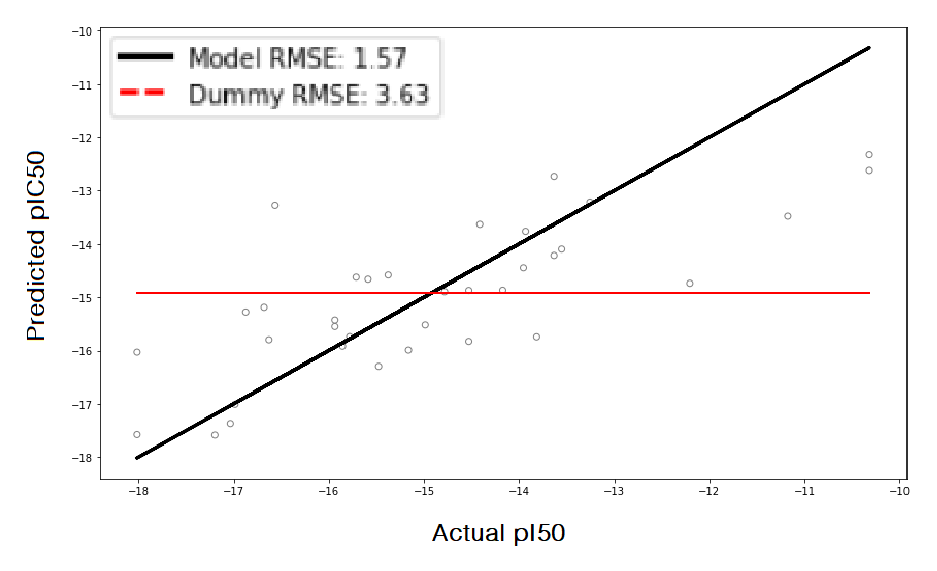
\includegraphics[width=0.6\textwidth]{Images/Results/dummy.png}
    \caption{Performance comparison of the dummy and Random Forest models.}
\end{figure}


